%% v3.0 [2015/11/14]
%\documentclass[Proof,technicalreport]{ieicej}
\documentclass[technicalreport]{ieicej}
%\usepackage{graphicx}
\usepackage[T1]{fontenc}
\usepackage{lmodern}
\usepackage{textcomp}
\usepackage{latexsym}
%\usepackage[fleqn]{amsmath}
%\usepackage{amssymb}
%\usepackage[dvipdfmx]{hyperref}
\usepackage{url}
\def\IEICEJcls{\texttt{ieicej.cls}}
\def\IEICEJver{3.0}
\newcommand{\AmSLaTeX}{%
 $\mathcal A$\lower.4ex\hbox{$\!\mathcal M\!$}$\mathcal S$-\LaTeX}
%\newcommand{\PS}{{\scshape Post\-Script}}
\def\BibTeX{{\rmfamily B\kern-.05em{\scshape i\kern-.025em b}\kern-.08em
 T\kern-.1667em\lower.7ex\hbox{E}\kern-.125em X}}
\jtitle{初級学習者を対象としたアラビア語検索サイトの構築}
\etitle{Construction of an Arabic searching website for beginner-level learners}
\authorlist{%
 \authorentry[inoue.kai.n0@tufs.ac.jp]{井上 開}{Kai INOUE}{Tokyo}% 
 \authorentry[sano@tufs.ac.jp]{佐野 洋}{Hiroshi SANO}{Tokyo}% 
}
\affiliate[Tokyo]{東京外国語大学言語文化学部\hskip1zw
  〒183-8534 東京都府中市朝日町3-11-1}
 {Faculty of Engineering,
  Tokyo University of Foreign Studies\hskip1em
  Yamada 1--2--3, Minato-ku, Tokyo,
  105--0123 Japan}
\affiliate[Tokyo]{東京外国語大学大学院総合国際学研究院\hskip1zw
  〒183-8534  東京都府中市朝日町3-11-1}
 {R\&D Division, Osaka Corporation\hskip1em
  Kawada 4--5--6, Suita-shi,
  565--0456 Japan}
%\MailAddress{$\dagger$hanako@denshi.ac.jp,
% $\dagger\dagger$\{taro,jiro\}@jouhou.co.jp}
\begin{document}
%\novocalize
\begin{jabstract}
アラビア語は国連公用語の1つであり,全世界に3億人近い話者がいるといわれる.
日本ではまだまだ馴染みの薄いアラビア語だが,アラブ世界への社会的,経済的関心は着実に高まってきている.
これに合わせ,日本でのアラビア語学習環境の整備を進めていくことは必須である.
このような背景を踏まえ,筆者はアラビア語学習教材の作成に着手した.
本稿では,初級学習者を対象としたアラビア語検索サイト構築にいたる過程について説明する.
初級学習者を対象としたのには,2つの理由が挙げられる.
第一に,アラビア語学習者の一人として,教材の不足が理由で著者自身が学習初期に非常に苦労したこと.
第二に,日本におけるアラビア語学習者の大半が初級レベルにあることである.
検索サイトは,電子媒体特有の機能を備えている.
それは,アルファベット配列と語根配列の両立である.
アラビア語の辞書は伝統的に語根配列が採用されてきたが,初級学習者には使いこなすのが難しい.
同時に,語根配列によるメリットも数多く存在する.
紙媒体の辞書では二つの配列を同時には採用できないというジレンマを,電子媒体で辞書をつくることで解消している.
\end{jabstract}
\begin{jkeyword}
アラビア語
\end{jkeyword}
\begin{eabstract}
Arabic is one of the official languages of the United Nations, and it is said that there are nearly 300 million Arabic speakers all over the world. 
Although Arabic is still unfamiliar here in Japan, social and economic interest to the Arabic world has been steadily increasing in recent years. 
In according with this situation, it is essential to promote a development of Arabic learning environment in Japan.
Based on the above, I started to prepare an Arabic learning material. 
In this paper, I will explain a process of how I got on to build an Arabic searching website for beginner-level learners. 
There are two reasons why I targeted beginners. 
First of all, as one of Arabic learners, my own difficulty in the beginning was due to the lack of teaching materials. 
Secondly, most Arabic learners in Japan are at the beginner-level.
The searching website has a function characteristic of an electric medium. 
It is a compatibility between an alphabet sequence and a root sequence.
An Arabic dictionary traditionally adopted the root sequence, but it is difficult for beginner-lever learners to use. 
At the same time, there are some merits to adopt the root sequence. 
By making a dictionary in an electric media, I eliminated this dilemma that we cannot adopt these two sequences at the same time.
\end{eabstract}
\begin{ekeyword}
p\LaTeXe\ class file, typesetting
\end{ekeyword}
\maketitle
\section{はじめに}
近年,日本ではアラビア語の学習需要が高まりつつある.
2011年,防衛省はアラビア語圏への留学派遣を開始し\cite{nikkei},2012年には東京外国語大学がアラビア語専攻の学部生募集定員を15名から30名へと増員した.
これらの背景には,日本おける21世紀以降のアラブ地域に対する政治的・経済的関心の高まりがある.
政治的には,2001年の「9.11」を始め,2003年からの「イラク戦争」,2010年からは「アラブの春」,翌年には「シリア内戦」の勃発,また「イスラム国」によるテロの脅威は現在も続いており,2014年にはシリアのアレッポで日本人2名が拘束された.
経済的には,原油輸入先第1位がサウジアラビア,第2位がアラブ首長国連邦,両国からの輸入量を合わせると全体の約6割を占めている\cite{teikoku}.
また日本企業の湾岸地域への進出も盛んである.
日本貿易振興機構が調査を始めた2005年から2014年の間に,アラブ首長国連邦にある日系企業拠点数は2倍以上の431事業所にまで増加している\cite{jetro}.
2020年にはドバイでの万国博覧会の開催が決定しており,湾岸地域はこれからますます経済的盛り上がりをみせると予想される.

しかし,日本でのアラビア語学習環境はいまだ整っていない.
アラビア語を専門に学習できる大学は,東京外国語大学と大阪大学のみである.
鷲見\cite{washimi2016}らによれば,2014年度にアラビア語の授業が開講されている大学は48あり,そのうち専門に学習できる教育課程が存在するのは大阪大学と東京外国語大学のみであり,残りの46の大学では副専攻の外国語として授業が開講されている.
そのため現在日本の高等教育機関でアラビア語を学習する人口のほとんどが初級レベルにあるが,初学者用の学習教材は数が少ない.
特に辞書は初級を銘打っているものは数が少ない.
しかし紙媒体の辞書であるために基本形からしか語彙を調べることができず,語根を用いて語彙を調べることによる学習効果が期待できない.一方,これらの問題を解決した電子媒体の辞書は存在するものの,初学者向けに語彙が厳選されていない点や,スマートフォンでの利用に特化されていないなどの問題がある.

本研究では,『『大学のアラビア語』』単語帳』および『A Frequency Dictionary of Arabic』のデータを用いて,アラビア語辞書検索サイトを構築した.基本形からの検索と語彙検索とを両立させつつ,これらのデータを用いて語彙を初級者向けに厳選した.またスマートフォンからの利用に最適化したプラットフォームにすることで利便性を追求した.

\section{アラビア語の言語的特徴}
アラビア語は,アフロ・アジア語族のセム語派に属する言語である.アラビア語はエジプトやシリアをはじめ,20以上の国および地域で公用語となっている.
Ethnologue\footnote{\url{https://www.ethnologue.com/statistics/size}}によると,話者総人口はおよそ3億人にものぼると言われ,6つある国連公用語の1つにも数えられる.
またアラビア語はイスラム教の聖典であるコーランの言語であり,全世界およそ16億人のイスラム教徒が存在することを考慮に入れると,実に世界人口の5人に1人がアラビア語と関わりを持っていることとなる.

文字はアラビア文字を用い,右から左に向かって記述する一方,数字は逆に右から左に記述される.
28の子音が存在し,中でも咽頭化ないし軟口蓋音化した子音が特徴的である.
母音は/a/,/i/,/u/の短母音とそれぞれの長母音,また/ai/,/au/などの二重母音が弁別される.
文構造はVSO型が基本だが,SVO型を取ることも多い.
名詞と形容詞は格(主格,属格,体格)・性(男性,女性)・数(単数,双数,複数)によって変化し,定冠詞によって限定と非限定が区別される.
また複数形には規則形が存在するが,不規則変化するものが多数である.
名詞と形容詞では,単数形が辞書の見出し語となる基本形である.
動詞は人称(一人称,二人称,三人称)・性・数,および完了と非完了によって変化する.
動詞では,三人称男性単数完了形が辞書の見出しとなる基本形である.

アラビア語の語は,語根を派生して生成される.
語根とは,基本的な意味を持つ最小単位のことであり,西原\cite{nishihara2012}は「語から派生接辞と屈折接辞を取り除いた部分」と説明している.
アラビア語の語根は,一般的な意味での語根からさらに母音が取り除かれた部分のことを指す.
またアラビア語の語根は,その全ての派生語によって共有される抽象的な意味を示している\cite{habash2010}.

\begin{table}[ht]
\begin{center}
\begin{tabular}{l|cc}
   語根& <b>-<t>-<k> \textit{\textbf{k-t-b}} & 書くこと\\
  \hline
 派生語& <kAtibuN>  \textit{\underline{\textbf{k}}A\underline{\textbf{t}}i\underline{\textbf{b}}\~u}& 作家\\
  派生語& <kitAbuN>  \textit{\underline{\textbf{k}}i\underline{\textbf{t}}Aa\underline{\textbf{b}}\~u} & 本\\
\hline
\end{tabular}
\caption{***** ***** ***** ***** *****.}
\ecaption{***** ***** ***** ***** *****.}
\label{table:alignment}
\end{center}
\end{table}

例えば,「KāTiB」は「作家」を意味し,「KiTāB」は「本」を意味する.
両単語の語根は「KTB」であり,これは「書くこと」にまつわる語根である.
ここで注意したいのは,語根はその並べ方まで含めたものであり,語根「KTB」は,「BKT」や「KBT」 とは異なるということだ.
厳密に言えば,3子音の組み合わせではなく,3子音の順列であると言える.
また稀に2子音や4子音の語根も存在する.

\section{アラビア語辞書検索システムの構築}
\subsection{既存辞書の問題点}
紙媒体の初学者用の辞書としては,「パスポート初級アラビア語辞典」がある.
これは約4,200語を収録した基本形から検索する辞書である.
意味の選定や補足が従事している辞書であるが,辞書の利用しやすさをとって基本形からの検索採用したことで,後述する語根からの検索によって期待される学習効果が得られない.

一方,語根からの検索と基本形からの検索を両立させることのできる電子媒体の辞書としては「アラビア語検索エンジン アラジン\footnote{http://www.linca.info/alladin/}」が有名である.
語根からの検索と基本形からの検索を兼ね備えているだけでなく,動詞活用形や名詞複数形からも語彙を検索することができる.
しかし,莫大な語彙データを収録しており,それらを列挙する形で検索結果が表示されるため,必ずしも利用者が探している語彙とのマッチがとられるわけではない.
つまり莫大な語彙を収録しているがために,語彙データが厳選されていないという問題がある.

またパソコンからの利用に最適化されているため,スマートフォンの小さい画面では利用しづらいという問題もある.
LINEの調査によれば,日常的にインターネットを利用する際,85\%の人がスマートフォンを利用しており,そのうちスマートフォンのみを利用している人の割合は全体の約半数にも及ぶ.
特に若年層ではその傾向が如実である.
大学でアラビア語を学習する人の大半は,10代と20代であると考えられるため,アラビア語辞書検索サイトを使う際はスマートフォンから利用していると推測される.
学習者のインターネット利用環境に最適化させることが,課題の1つとなる.

\subsection{語根・基本形からの検索}
\subsubsection{語根からの検索}
伝統的にアラビア語の辞書では,語根から語彙を検索する辞書が主流であった.
表1の例であれば,「KāTiB」と「KiTāB」はともに辞書の見出し語「KTB」のグループにまとめられている.
今まで基本形から語彙を検索する日本語や英語の辞書しか使ったことのない学生が,語根から検索するアラビア語辞書の利用に慣れるまでには時間を要する.
語根から語彙を検索するためには,調べたい語彙の語根を判別する必要性があるからである.
これには相応の文法力が必要とされる.

\begin{table}[ht]
\begin{center}
\begin{tabular}{l|cc}
   語根& KTB & 書くこと\\
  \hline
 派生語& maKTaBaTun & 図書館\\
\hline
\end{tabular}
\caption{***** ***** ***** ***** *****.}
\ecaption{***** ***** ***** ***** *****.}
\label{table:alignment}
\end{center}
\end{table}

例えば,「maKTaBat」を辞書で引く場合,「m」と「t」がそれぞれ語根ではなく,派生語を作るための接辞であると見抜けなければならない.
これは簡単な例であるが,語根の中には派生された語彙において3子音のうち一部が脱落したり,変化したりするものがある.
これらは例外だが,使用頻度の高い重要語にも数多く見られる.

\begin{table}[ht]
\begin{center}
\begin{tabular}{l|cc}
   語根& NWM & 寝ること\\
  \hline
 派生語& NāMa & 寝た\footnote{三人称男性単数完了形}\\
  派生語& NiYāM & 睡眠\\
\hline
\end{tabular}
\caption{***** ***** ***** ***** *****.}
\ecaption{***** ***** ***** ***** *****.}
\label{table:alignment}
\end{center}
\end{table}

「NWM」は「寝る」に関わる語根だが,これが派生した動詞「NāMa」では第二子音「W」が長母音化し,名詞「NiyāM」では同じく第二子音「W」が「Y」に変化している.
これらの例のように,一見しただけでは語根の判別が難しい語彙も多い.
こういった場合,語根から辞書を引くことは格段に難しくなる.
特に文法力がまだ十分に備わっていない初学者は,語彙の意味を調べることさえできないという状態に陥る.
これが語根を用いて検索する辞書の大きなデメリットである.
しかし,逆に語根を正しく判別するだけの文法力さえあれば,同じ語根から派生された語彙群を一覧することができるというメリットもある.
「KTB」を引けば,「作家」,「本」,「図書館」という語彙を同時に知ることができる.
また動詞の活用形や名詞・形容詞の複数形を基本形に戻すことができないとしても,語根から辞書を引くことで意味を知ることが可能である.

\begin{table}[ht]
\begin{center}
\begin{tabular}{l|ccc}
   語彙 & 意味 & 複数形\\
  \hline
 KāTiBun & 作家 & KuTTāBun \\
  KiTāBun & 本 & KuTuBun\\
\hline
\end{tabular}
\caption{***** ***** ***** ***** *****.}
\ecaption{***** ***** ***** ***** *****.}
\label{table:alignment}
\end{center}
\end{table}

語根から引く辞書であれば,「KuTTāBun」が「KāTiBun」の複数形 であると知らなくとも,語根が「KTB」であるということさえわかれば,辞書を引いて意味を知ることできる.
「KuTuB」に関しても同様であり,これらの語彙はいずれも語根に対して母音が付加されているだけなので,語根の判別は難しくない.
それゆえ語根から引く辞書であれば,たとえこれらの語彙が初見であったとしても辞書を引くことは十分に可能である.

\subsubsection{基本形からの検索}
語根から検索する辞書がある一方で,日本語や英語の辞書と同様に基本形から検索する辞書も存在する.
この場合,調べたい語彙の語根を判別できる文法能力は必要とならないため,初学者にとっては使い勝手がよいというメリットがある.
「NWM」のように派生語において語根の一部が,欠落および変化してしまう語彙も,単純にそのままの形で調べれば良いだけである.
しかし一点注意しなければいけないことがある.
名詞・形容詞は単数形,動詞は三人称男性単数完了形が基本形となっているため,調べたい語彙が名詞・形容詞の複数形だった場合や,動詞の活用形だった場合や,それらを基本形に戻す文法力が必要である.

表4の例であれば,「KuTTāB」は「KāTiB」に,「KuTuB」は「KiTāB」に戻さなければ辞書を引くことはできない.
複数形が規則変化するものである場合,複数形から単数形を復元することはさして難しくないため,アルファベット配列の辞書ですぐに調べることができる.
しかし例に挙げた名詞のように複数形が不規則変化するものの場合,辞書を引くのは当然それらが学習者にとって初見の時であるため,複数形から単数形への復元は困難であり,辞書を引くことは難しくなる.
この場合には,語根から検索する方が適当である.
また同じ語根から派生された語彙群を一覧することができないため、辞書を引くという行為が新たな語彙を学ぶという部分に結びつかない。初学者にとって語根から検索することは難しいが,同時に多くの語彙を覚えなければいけない学習初期にこそ語根から語彙を調べることが効率的である.

\subsubsection{検索方法の検討}
語根検索と基本形検索にはそれぞれに長所と短所がある.

語根検索には,同じ語根から派生した語彙を一覧できることや,語彙を基本形に戻せなくても検索できるといったメリットが存在する.
特に前者に関しては,語彙を調べつつ,新たな語彙を学ぶことができ,高い学習効率が期待できる.
一方で語彙の語根を見抜く文法力が要求されることが最大のデメリットである.
これは初学者にとって大きな障壁となる.

基本形検索では,語根に関する知識がなくても辞書を利用できるため,初学者にも利用しやすいことが最大のメリットとなる.
しかし,今度は語彙を基本形に戻せるだけの文法力が要求される.

使いやすさのみを考慮すれば,基本形検索を採用することが妥当であるが,語根引きによって得られる学習効果も大きい.アラビア語辞書において伝統的に語根引きが採用されてきたことは,語根に対する理解がアラビア語学習において非常に重要であるからに他ならない.しかし榮谷\cite{sakaedani2008}も指摘するように,語根を重視して文法学習に重点をおけば,かえって語彙を覚える時間が取れなくなる可能性もある.

紙媒体の辞書では,物理的にどちらか一方の検索方法しか採用できないため,目的に応じて使い分けようとすれば2冊必要となってしまう.
他方電子媒体の辞書であれば両方を採用することができる.
電子媒体の辞書をつくることの最大のメリットは,この点にある.
本論で構築する辞書検索サイトも語根検索と基本形検索を備えている.

\subsection{アラビア語辞書データ}
我々は,収録する語彙データとして『『大学のアラビア語』』単語帳』より2081語を抽出した.
これは,大学でアラビア語を学ぶ人が覚えるべき語彙を収録したものである.
さらに『A Frequency Dictionary of Arabic』の上位2000語のうち,『『大学のアラビア語』』単語帳』に含まれない818語を追加した.
最終的に全2909語を収録した.
またTUFS言語モジュール\cite{kawaguchi2007}にアップロードされている約2000文を例文として収録した.

3.1で取り上げたように,語彙数をむやみに増やせば初学者にとって検索結果の中から適切なものを選び出すのが困難となる.
では初学者にとって最低限必要となる語彙数はどの程度の量になるのか.
第二言語習得においてどれだけの語彙量を目標にすべきかに関して,Nation [3]は語彙の頻度に注目することを1つの方法として挙げている.
彼は英語ネイティブスピーカーの中等学校教科書を例に,最も頻度の高い2000語でテキストの87\%,さらにUniversity word list を加えた2800語でテキストの95\%をカバーしていると示している.
この結果は英語に限られるものであり,他言語にも同じように頻度とテキストカバー率の関係を当てはめるべきではない.

しかしTim Buckwalter・Dilworth Parkinson [4]が,語彙学習において頻度を1つの指標とした際,多くの場合学習者の利益となる語彙表を得られると述べているように,頻度が重要な指標となることは間違いない.
とりわけ「初級学習者がまず学ぶべき語彙を提示する」という条件のもとでは,効果的だと考えられる.

\subsection{実装詳細}
辞書検索サイトには,基本形検索,語根検索,および日本語検索が備わっている.

\begin{figure}[htbp]
 \begin{center}
  \fbox{
  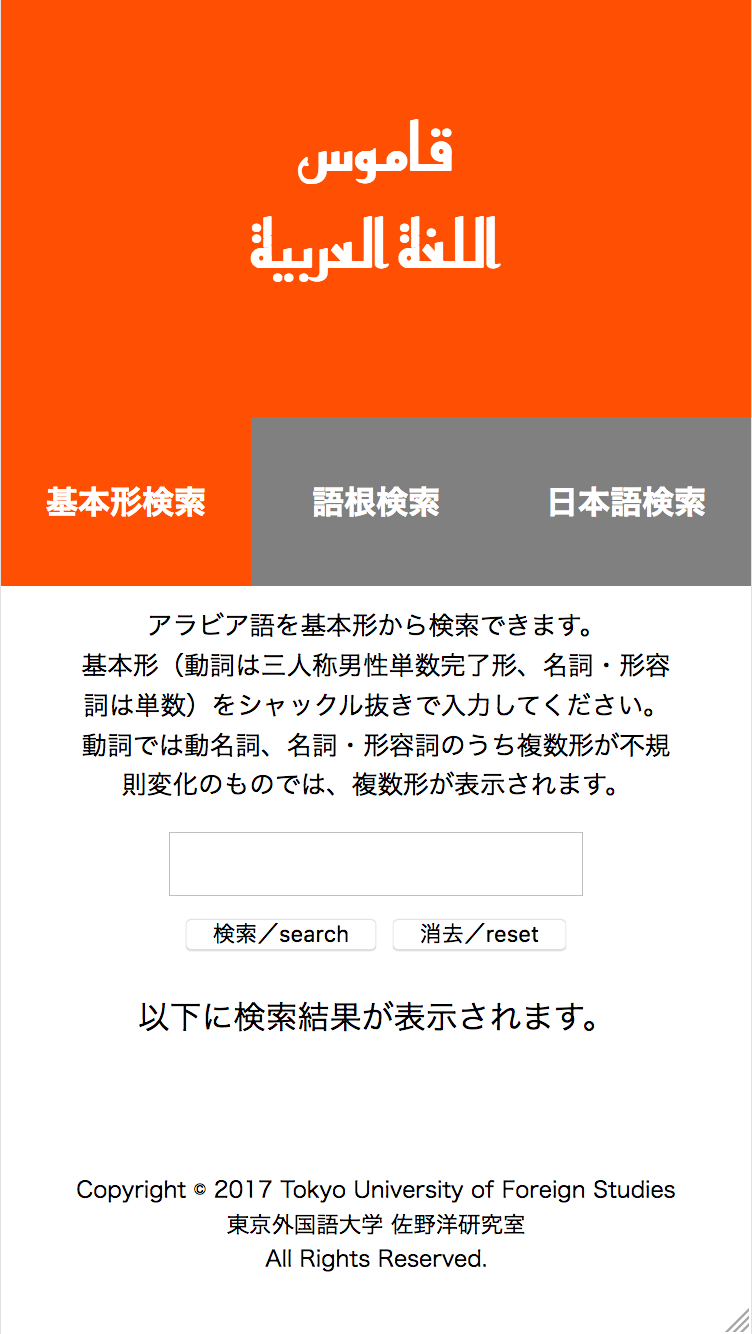
\includegraphics{fig01.png}
  }
 \end{center}
 \caption{表1}
 \label{fig:one}
\end{figure}

\begin{thebibliography}{99}
\bibitem{washimi2016}
鷲見朗子 鷲見克典, 日本の高校と大学におけるアラビア語の教育と学習者, アラブ・イスラム研究(14), pp.103-121, 2016.
\bibitem{habash2010}
Nizal Y. Habash,Introduction to Arabic Natural Language Processing,Morgan\&Claypool,2010
\bibitem{nishihara2012}
西原哲雄,言語学入門,朝倉書店,2012
\bibitem{sakaedani2008}
榮谷温子, アラビア語辞典の語根順配列とアルファベット順配列語彙習得の観点から, 外国語教育研究(11), pp.90-100, 2008.
\bibitem{heinle1990}
I.S.P.Nation,Teaching and Learning Vocabulary, Heinle\&Heinle, 1990. 
\bibitem{buckwalter2009}
Tim Buckwalter  Parkinson Dilworth, A Frequency Dictionary of Arabic: Core Vocabulary for Learners, Routledge, 2009.
\bibitem{kawaguchi2007}
Yuji Kawaguchi,Toshihiro Takagaki,Nobuo Tomimori,and Yoichiro Tsuruga,
Corpus-Based Perspectives in Linguistics,John Benjamins
\bibitem{teikoku}
帝国書院, \url{https://www.teikokushoin.co.jp/statistics/map/index16.html.}.
\bibitem{jetro}
JETRO, \url{https://www.jetro.go.jp/ext_images/_Reports/02/8a510d662cfc29f9/6_jpcompany. pdf}.
\bibitem{nikkei}
日本経済新聞, \url{https://www.nikkei.com/article/DGXNZO22129830T20C11A1PE8000/}.
\end{thebibliography}
\end{document}